\documentclass[twocolumn]{article}
\usepackage{booktabs}
\usepackage{listings}
\usepackage{xcolor}
\usepackage{geometry}
\geometry{margin=1in}
\usepackage{amsmath}
\usepackage{graphicx}
\usepackage{float}
\usepackage{moresize}

\usepackage[backend=biber,style=authoryear]{biblatex} % Choose your style
\addbibresource{references.bib} % Use the name of your .bib file
    

\definecolor{codegray}{gray}{0.9}
\definecolor{deepblue}{rgb}{0,0,0.5}
\definecolor{deepred}{rgb}{0.6,0,0}
\definecolor{deepgreen}{rgb}{0,0.5,0}

\lstdefinestyle{mypython}{
    backgroundcolor=\color{codegray},   
    commentstyle=\color{deepgreen},
    keywordstyle=\color{deepblue},
    numberstyle=\tiny\color{gray},
    stringstyle=\color{deepred},
    basicstyle=\ttfamily\footnotesize,
    breakatwhitespace=false,         
    breaklines=true,                 
    captionpos=b,                    
    keepspaces=true,                 
    numbers=left,                    
    numbersep=5pt,                  
    showspaces=false,                
    showstringspaces=false,
    showtabs=false,                  
    tabsize=4,
    language=Python
}


% Custom author info
\pagenumbering{gobble}
\title{
    \textbf{\small COMS4047A}\\[0.5em]
    \textbf{Reinforcement Learning}\\[1em]
    {\Huge \textbf{Assignment}}\\[3cm]
    
\includegraphics[width=0.4\textwidth]{download.png}
}

\author{
    \small
    \begin{tabular}{l}
    \textbf{Taboka Chloe Dube - 2602515} \\
    \textbf{Wendy Maboa - 2541693} \\
    \textbf{Liam Brady - 2596852} \\
    \textbf{Refiloe Mopeloa - 2333776}
    \end{tabular}
}

\begin{document}

\begin{titlepage}  % <- ensures it's treated as a full separate page
    \maketitle
\end{titlepage}


\newpage

\pagenumbering{arabic} 
\setcounter{page}{1}
\section*{Introduction}
Crafter is a procedurally generated 2D survival game designed as a benchmark for reinforcement learning
 research. It features a diverse set of tasks including resource gathering, tool crafting, creature combat, and
 achievement hunting, all while managing survival mechanics like hunger and health. This report will provide an overview of implementation of agents in Crafter using DQN and PPO algorithms.

\section*{In-class Algorithm: DQN}

\section*{Out-of-class Algorithm: PPO}

PPO (Proximal Policy Optimization) is a reinforcement learning algorithm that trains an agent by optimizing its decision-making policy. It works by collecting data through interactions with an environment and then using a clipped objective function to make stable updates to the policy. This approach is known for being more stable, efficient, and easier to implement than some other policy gradient methods \parencite{schulman}.

\subsection*{Motivation}
PPO (Proximal Policy Optimization) is a good choice for the Crafter environment because it provides a strong balance of stability, sample efficiency, and simplicity while effectively handling the environment's key challenges, such as sparse rewards, long-term reasoning, and procedural generation. 

In addition these are the following theoretical benefits of PPO:
\begin{itemize}
    \item \textbf{Stable Policy Updates:} The Crafter environment is complex and dynamic, where large, unconstrained policy updates could easily destabilize training and cause the agent to forget beneficial behaviors. PPO's clipping mechanism limits how much the policy can change at each step, ensuring stable and controlled learning.
    \item \textbf{Sample Efficiency:} Crafter involves many different achievements and complex interactions, meaning efficient use of experience is crucial. PPO is relatively sample-efficient because it can reuse collected data over multiple training epochs (mini-batches) without significant instability, unlike other on-policy methods that only use data once.
    \item \textbf{Facilitates Exploration:} The PPO objective often includes an entropy bonus term, which encourages the agent to explore different actions and strategies. This is vital in Crafter, which features wide, procedurally generated worlds and independent achievements that require broad exploration to discover all possibilities.
\end{itemize}

\subsection*{Baseline Implementation}
The baseline agent was implemented using the Stable-Baselines3 PPO algorithm. The initial hyperparameters were chosen to provide stable learning without aggressive updates, ensuring reproducibility. The agent at this point perceives the environment through single still images (frames) rather than continuous sequences, meaning it has only a limited view of the environment at each step.
\subsubsection*{Observations and Performance}
The baseline PPO agent exhibited some exploratory behavior and moderate learning progress. However, its limited temporal awareness significantly constrained performance. The average episodic reward stabilized around \textbf{3.26}, with the maximum reward achieved being \textbf{7.1}.
The following figures show the reward and survival distribution rates over 100 episodes:
\begin{figure}[H]
    \centering
    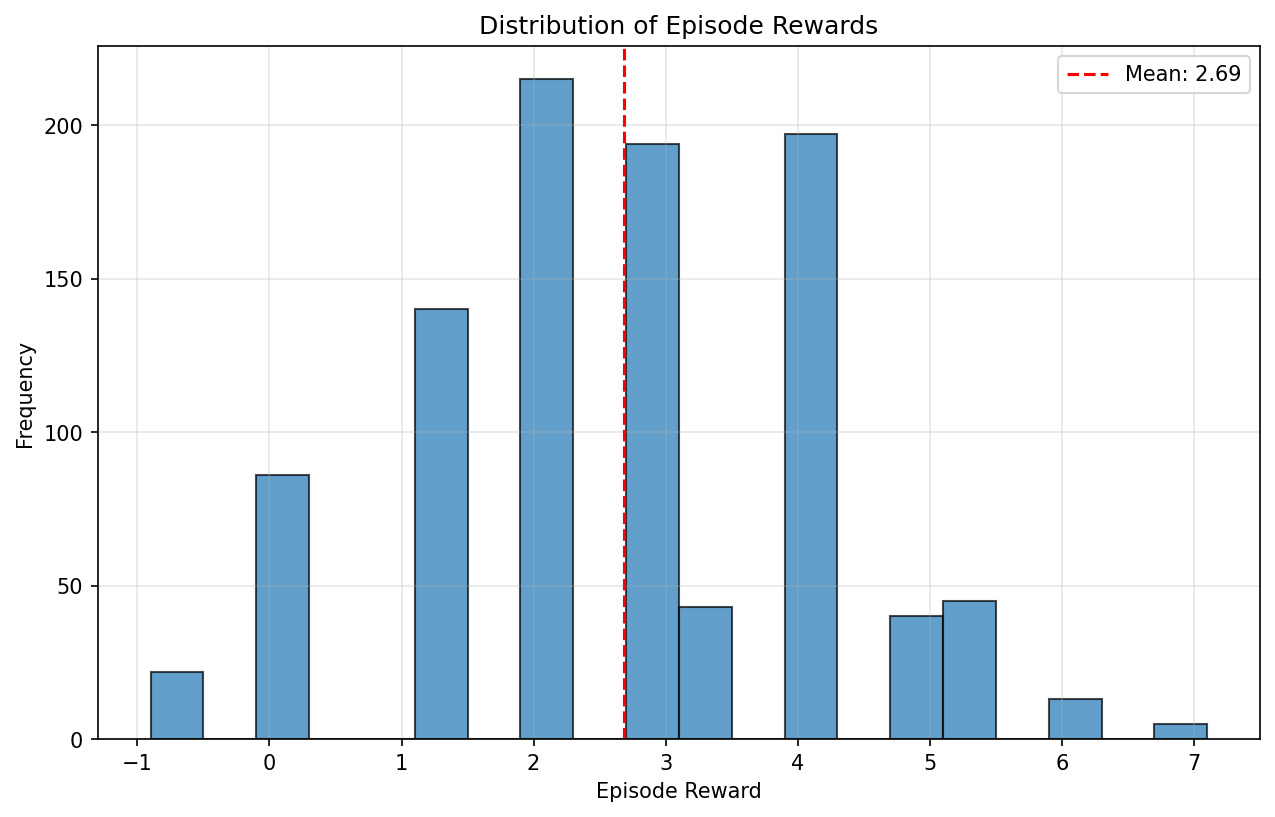
\includegraphics[width=0.75\linewidth]{images/reward_distribution_ppo_baseline.png}
    \caption{Reward distribution of PPO baseline}
    \label{fig:placeholder}
\end{figure}
\begin{figure}[H]
    \centering
    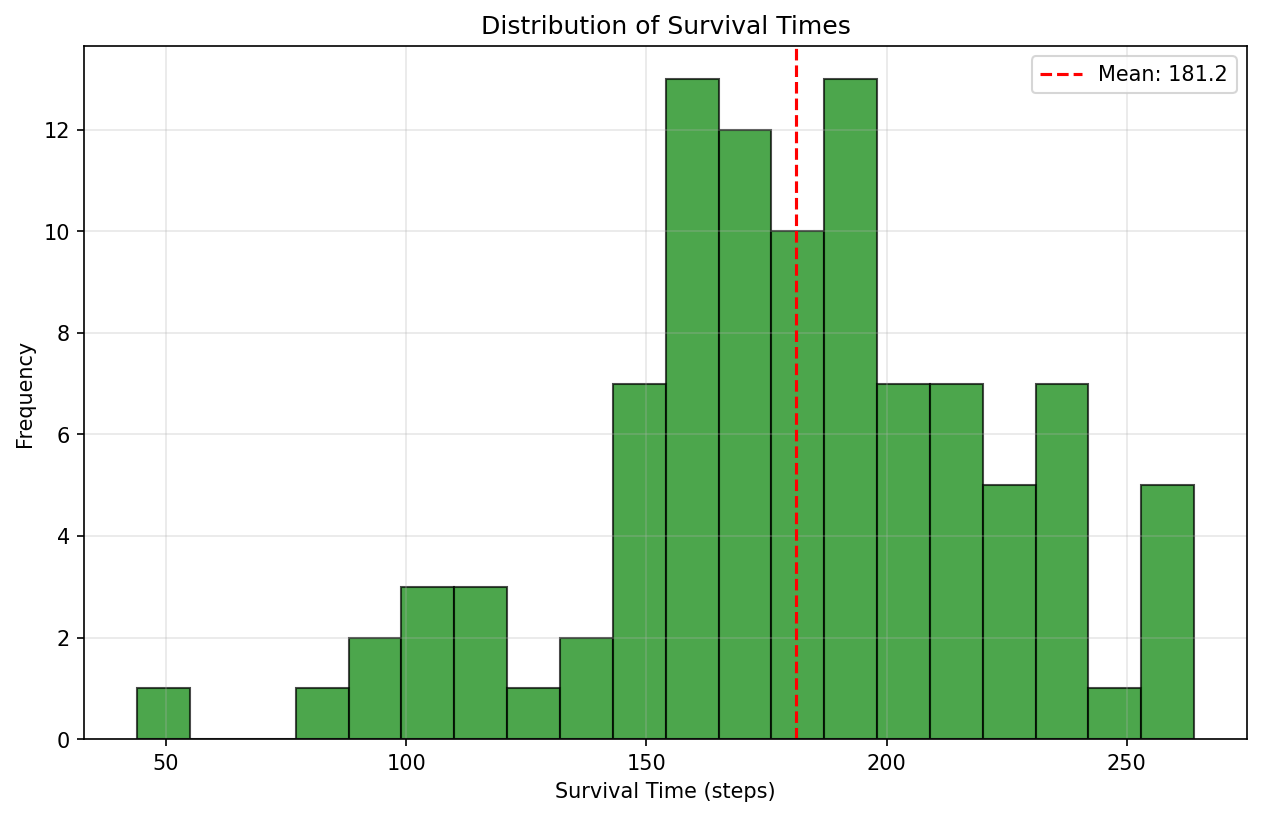
\includegraphics[width=0.75\linewidth]{images/survival_distribution_ppo_baseline.png}
    \caption{Survival distribution of PPO baseline}
    \label{fig:placeholder}
\end{figure}
\subsubsection*{Identified areas of improvement}
The following weaknesses were identified in the baseline model:
\begin{itemize}
    \item \textbf{Lack of Memory:} The agent cannot recall previous states or actions, leading to suboptimal long-term decision-making.
    \item \textbf{Limited Exploration:} Without memory or intrinsic motivation, exploration remained shallow, resulting in repetitive behavior.
\end{itemize}
\subsubsection*{Improvements and Methodology}
To address these issues, a Recurrent PPO (R-PPO) architecture was introduced. This variant augments the standard PPO with a recurrent neural network (RNN) layer, allowing the policy to maintain an internal state across time steps. This addition provides the agent with short-term memory, improving decision consistency under partial observability.

\subsection*{Improvement 1: Random Network Distillation}
\subsection*{Improvement 2: Long-Short Term Memory}

\subsubsection*{Improvement 2 Implementation}
To address the baseline limitations in memory and exploration, we implemented a \textbf{Recurrent Proximal Policy Optimization (Recurrent PPO)} agent. This model extends PPO by incorporating a Long Short-Term Memory (LSTM) layer, enabling the policy to retain temporal context across time steps. This memory mechanism helps the agent handle the partially observable nature of the Crafter environment, where important state information may not be visible in a single frame.
The hyperparameters were kept the same as the baseline to make sure that the LSTM implementation would show a decent improvement in comparison to the baeline.

Additonally, slight reward shaping was employed to accelerate convergence and guide exploration towards useful sub-goals. This ensured that intermediate achievements (such as crafting tools or collecting resources) contributed meaningful gradient signals during training.
\begin{figure}[H]
    \centering
    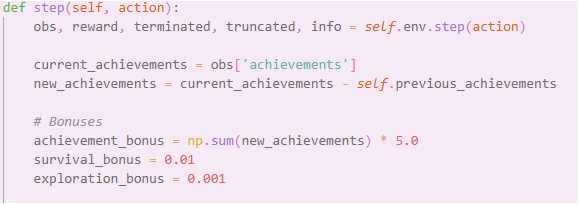
\includegraphics[width=0.5\linewidth]{images/RewardShaping.png}
    \caption{Reward Shaping implemented in RecurrentPPO agent}
\end{figure}

\subsubsection*{Observations and Performance}
The introduction of temporal recurrence through an LSTM notably improved the agent's ability to integrate information across time steps. Compared to the baseline PPO model, which achieved a mean episodic reward of approximately 3.26 (maximum 7.1), the Recurrent PPO (R-PPO) demonstrated consistent performance gains.

\subsubsection*{Qualitative Observations}

Behaviorally, the Recurrent PPO agent demonstrated:
\begin{itemize}
    \item More coherent decision sequences across time, owing to the LSTM's memory retention.
    \item Improved persistence in long-horizon tasks such as crafting and navigation.
    \item Less tendency to repeat suboptimal exploration patterns seen in the baseline agent.
\end{itemize}

In addition, reward shaping contributed to smoother early learning and faster convergence during training, as the agent received structured feedback for intermediate achievements.

\subsubsection*{Discussion}

The performance gain from incorporating temporal memory validates the hypothesis that Crafter's partial observability penalizes stateless architectures. By maintaining a hidden state, the Recurrent PPO agent effectively constructs an implicit representation of unobserved parts of the environment. This allows for more context-aware actions and ultimately leads to higher cumulative rewards. 

While the improvement is evident, the results also reveal that the agent has not fully stabilized—indicated by the wide reward range. Further tuning of learning rate, clipping threshold, and recurrent hidden size could reduce variance and enhance consistency across episodes.

The following figures show the different reward and survival distribution rates over 100 episodes:

\begin{figure}[H]
    \centering
    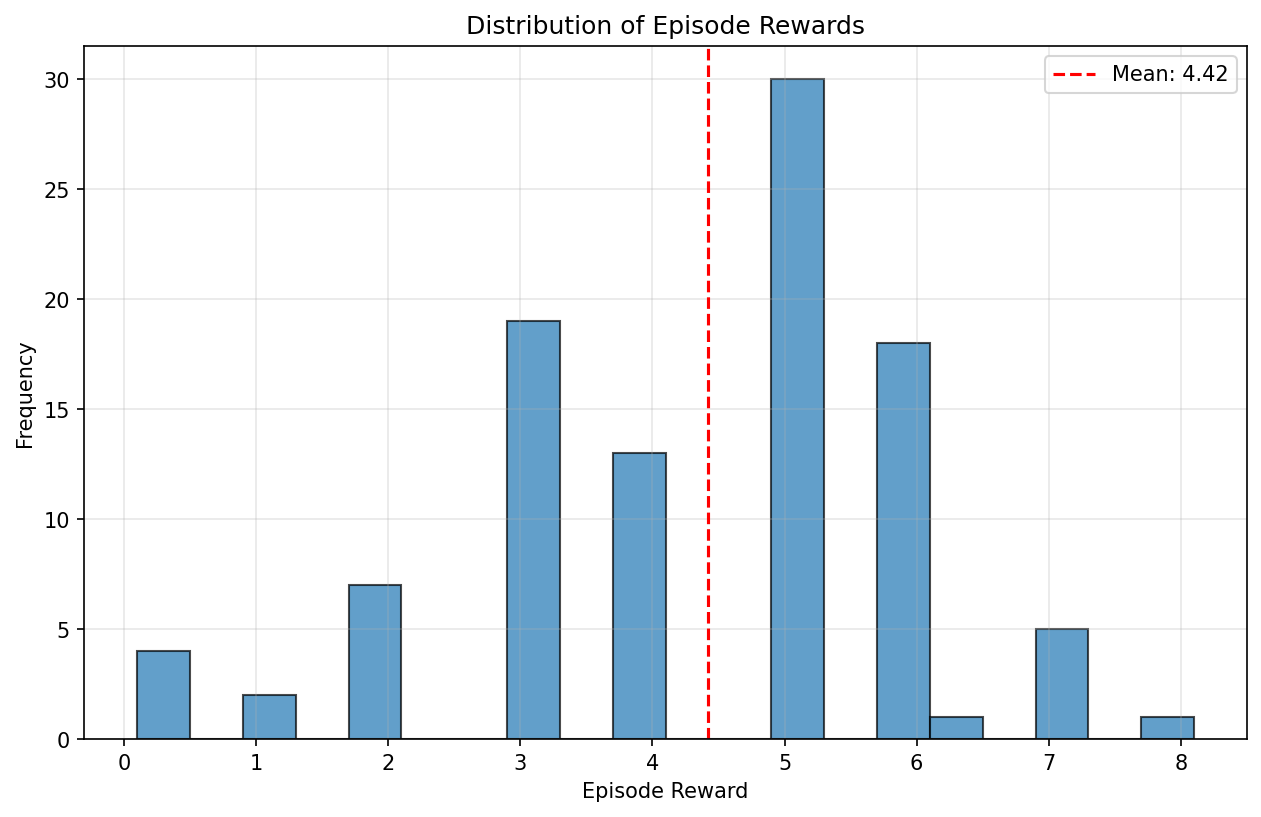
\includegraphics[width=0.75\linewidth]{images/reward_distribution_ppo_improv2.png}
    \caption{Reward distribution of PPO baseline}
    \label{fig:placeholder}
\end{figure}
\begin{figure}[H]
    \centering
    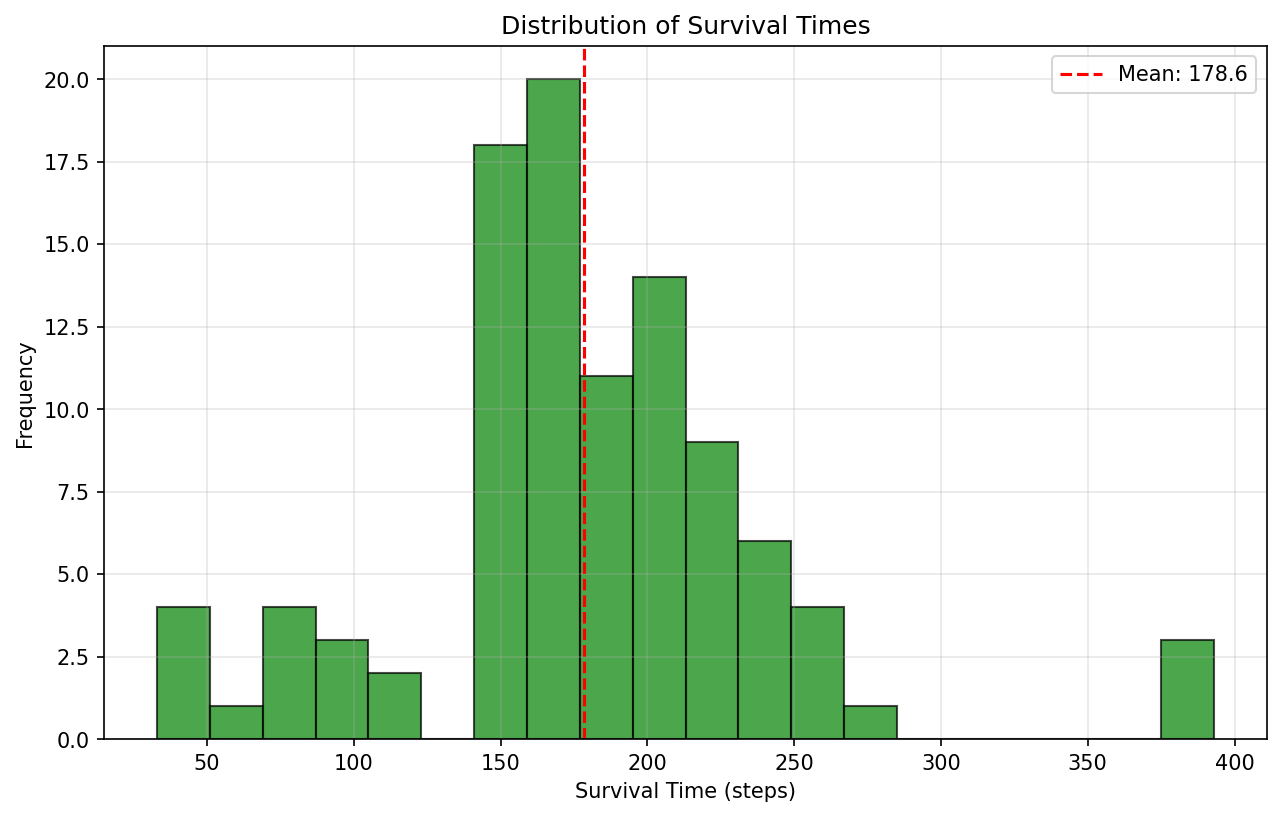
\includegraphics[width=0.75\linewidth]{images/survival_distribution_ppo_improv2.png}
    \caption{Survival distribution of PPO baseline}
    \label{fig:placeholder}
\end{figure}

An interesting observation from the experiments was that the Recurrent PPO (R-PPO) agent achieved a higher average reward (4.42) than the baseline PPO (3.26), despite exhibiting a lower overall survival rate. This contradiction can be explained by the agent's behavioral bias toward short-term, high-value actions.

The inclusion of memory through the LSTM layer allowed the agent to recall and exploit previously observed opportunities, such as nearby resources or enemies, resulting in higher reward density per timestep. However, this same decisiveness increased exposure to risk, reducing overall survival time.

Additionally, the use of reward shaping likely amplified this effect by reinforcing immediate sub-goal completion (e.g., crafting, combat) rather than conservative, long-term survival strategies. Consequently, the R-PPO learned to act more efficiently but less cautiously, prioritizing cumulative reward over lifespan duration.

This highlights a fundamental reinforcement learning trade-off between \textit{reward maximization} and \textit{survival optimization}, emphasizing that longer episodes do not necessarily equate to better task performance.




\end{document}
